\documentclass[12 pt, a4paper]{article}
\usepackage[utf8]{inputenc}
\usepackage[left=2.5 cm,top=2.54 cm,right=2.5 cm,bottom=2.54 cm]{geometry}
\usepackage[flushleft]{threeparttable}
\usepackage{mathtools}
\usepackage{amssymb}
\usepackage{amsmath}
\title{Linear Statistical Models Assignment 2}
\date{}
\usepackage[dvipsnames]{xcolor}
\usepackage{graphicx,wrapfig}
\author{Kim Seang CHY}
\usepackage{xcolor}
\usepackage{lipsum}
\usepackage{mwe}

%Table Adjustment
\usepackage{tabularx}
\newcommand{\tabitem}{~~\llap{\textbullet}~~}

\begin{document}

\maketitle

\noindent \textbf{Question 1:} Maximum likelihood of $\sigma^2$\\

\noindent \ Recall that in the general full model $\boldsymbol{\varepsilon} \sim MVN(0,\sigma^2I) $, hence the likelihood function is given by:\\
\begin{align*}
L(\beta,\sigma)&=\prod_{i=1}^n \frac{1}{\sqrt{2 \pi} \sigma} \text{exp} \left( \frac{-\varepsilon_{i}^2}{2 \sigma^2} \right) \\
 &=(2 \pi)^{-\frac{n}{2}} \sigma^{-n} \text{exp} \left(\sum_{i=1}^{n} \frac{-\varepsilon_{i}^2}{2 \sigma^2} \right)
\end{align*}

\noindent Let $\ell(\beta,\sigma)$ be the log likelihood function of $L(\beta,\sigma)$.

\begin{align*}
\ell(\beta, \sigma)= -\frac{n}{2} \log(2 \pi)-n\log(\sigma) -\frac{1}{2\sigma^2}\left(\sum_{i=1}^{n}\varepsilon_{i}^2 \right)
\end{align*}

\noindent Since $\sum_{i=1}^{n}\varepsilon_{i}^2=(\textbf{y}-\textbf{X}\boldsymbol{\beta})^{T}(\textbf{y}-\textbf{X}\boldsymbol{\beta})=SS_{Res}$:


\begin{align*}
&\ell(\beta, \sigma)= -\frac{n}{2} \log(2 \pi)-n\log(\sigma) -\frac{SS_{Res}}{2\sigma^2}\\
&\frac{\partial \ell}{\partial \sigma}=-\frac{1}{\sigma}+\frac{SS_{Res}}{\sigma^3}
\end{align*}

\noindent Setting $\frac{\partial \ell}{\partial \sigma}=0$ and solve for $\sigma$ we get:
\begin{align*}
-\frac{1}{\sigma}+\frac{SS_{Res}}{\sigma^3}=0\\
\implies \sigma=\frac{SS_{Res}}{n}
\end{align*}


\pagebreak

\noindent \textbf{Question 3:} Show that the $SS_{Res}$ for the first model is at least the $SS_{Res}$ for the second model. \\

\noindent For the second model our sum of residual is given by  $SS_{Res}=\textbf{y}^T\textbf{y}-\textbf{y}^T\textbf{Hy}=\textbf{y}^T\textbf{y}-\textbf{y}^T\textbf{X}\boldsymbol{\beta}$. Since $\textbf{Hy}=\textbf{X}\boldsymbol{\beta}$, then $SS_{Res}=\textbf{y}^T\textbf{y}-\textbf{y}^T\textbf{X}\boldsymbol{\beta}$\\ 

Let $SS_{Res_{\gamma_1}}=\textbf{y}^T\textbf{y}-\textbf{y}^T\textbf{H}_1\textbf{y}$ be the sum of residual of the first model.


\noindent We can partition $\textbf{X}$ and $\boldsymbol{\beta}$ as follow:\\

\noindent $\textbf{X}=
\left[
\begin{array}{c|c}
\textbf{X}_1 & \textbf{X}_2 \\
\end{array}
\right] $ and
$\boldsymbol{\beta}=
\left[
\begin{array}{c}
\boldsymbol{\gamma}_1 \\
\hline
\boldsymbol{\gamma}_2
\end{array}
\right] $ \\

\noindent Hence, $\textbf{X}\boldsymbol{\beta}=\textbf{X}_1\boldsymbol{\gamma}_1+\textbf{X}_1\boldsymbol{\gamma}_2=\textbf{H}_1\textbf{y}+\textbf{H}_2\textbf{y}$, where $\textbf{H}_1$ is the hat matrix the first model and $\textbf{H}_2$ is hat matrix for the rest of the predictor that was in the second model but not in first model.  Thus $SS_{Res}$ of the full model is given by: \\

\begin{align*}
SS_{Res}&=\textbf{y}^T\textbf{y}-\textbf{y}^T(\textbf{H}_1+\textbf{H}_2)\textbf{y} \\
&= \textbf{y}^T\textbf{y}-\textbf{y}^T\textbf{H}_1\textbf{y}-\textbf{y}^T\textbf{H}_2\textbf{y}\\
&=SS_{Res_{\gamma_1}}-\textbf{y}^T\textbf{H}_2\textbf{y}\\
\end{align*}

\noindent Since $\textbf{H}_2$ is an idempotent and symmetric matrix,  this implied its eigenvalue are either 0 or 1, hence it is positive semi-define,  implies $\textbf{y}^T\textbf{H}_2\textbf{y} \geq 0$.  Hence $SS_{Res_{\gamma_1}} \geq SS_{Res}$. 







\pagebreak
\textbf{e.} Produce diagnostic plots for your final model from stepwise selection and comment.

\begin{figure}[h]
    \centering
    \begin{minipage}{0.45\textwidth}
        \centering
        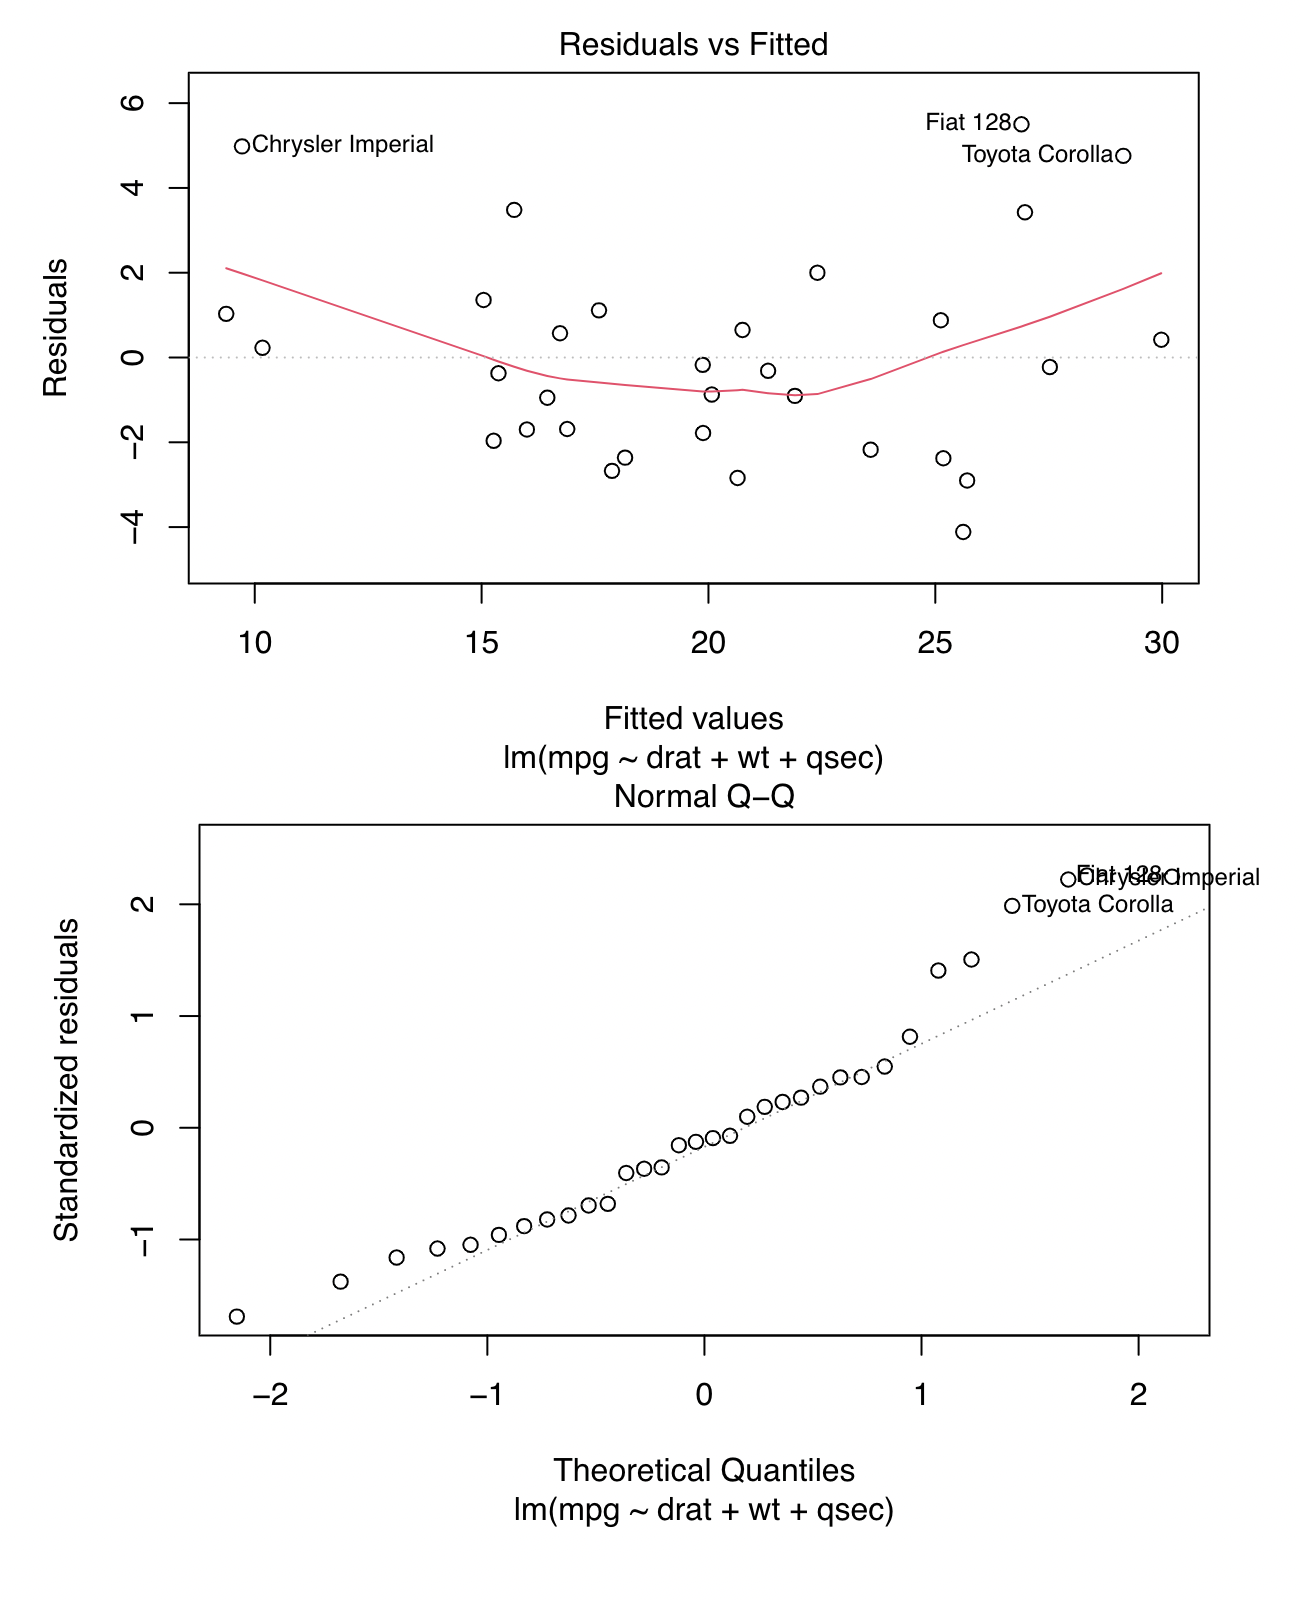
\includegraphics[width=0.9\textwidth]{Graph1} % first figure itself
    \end{minipage}\hfill
    \begin{minipage}{0.45\textwidth}
        \centering
        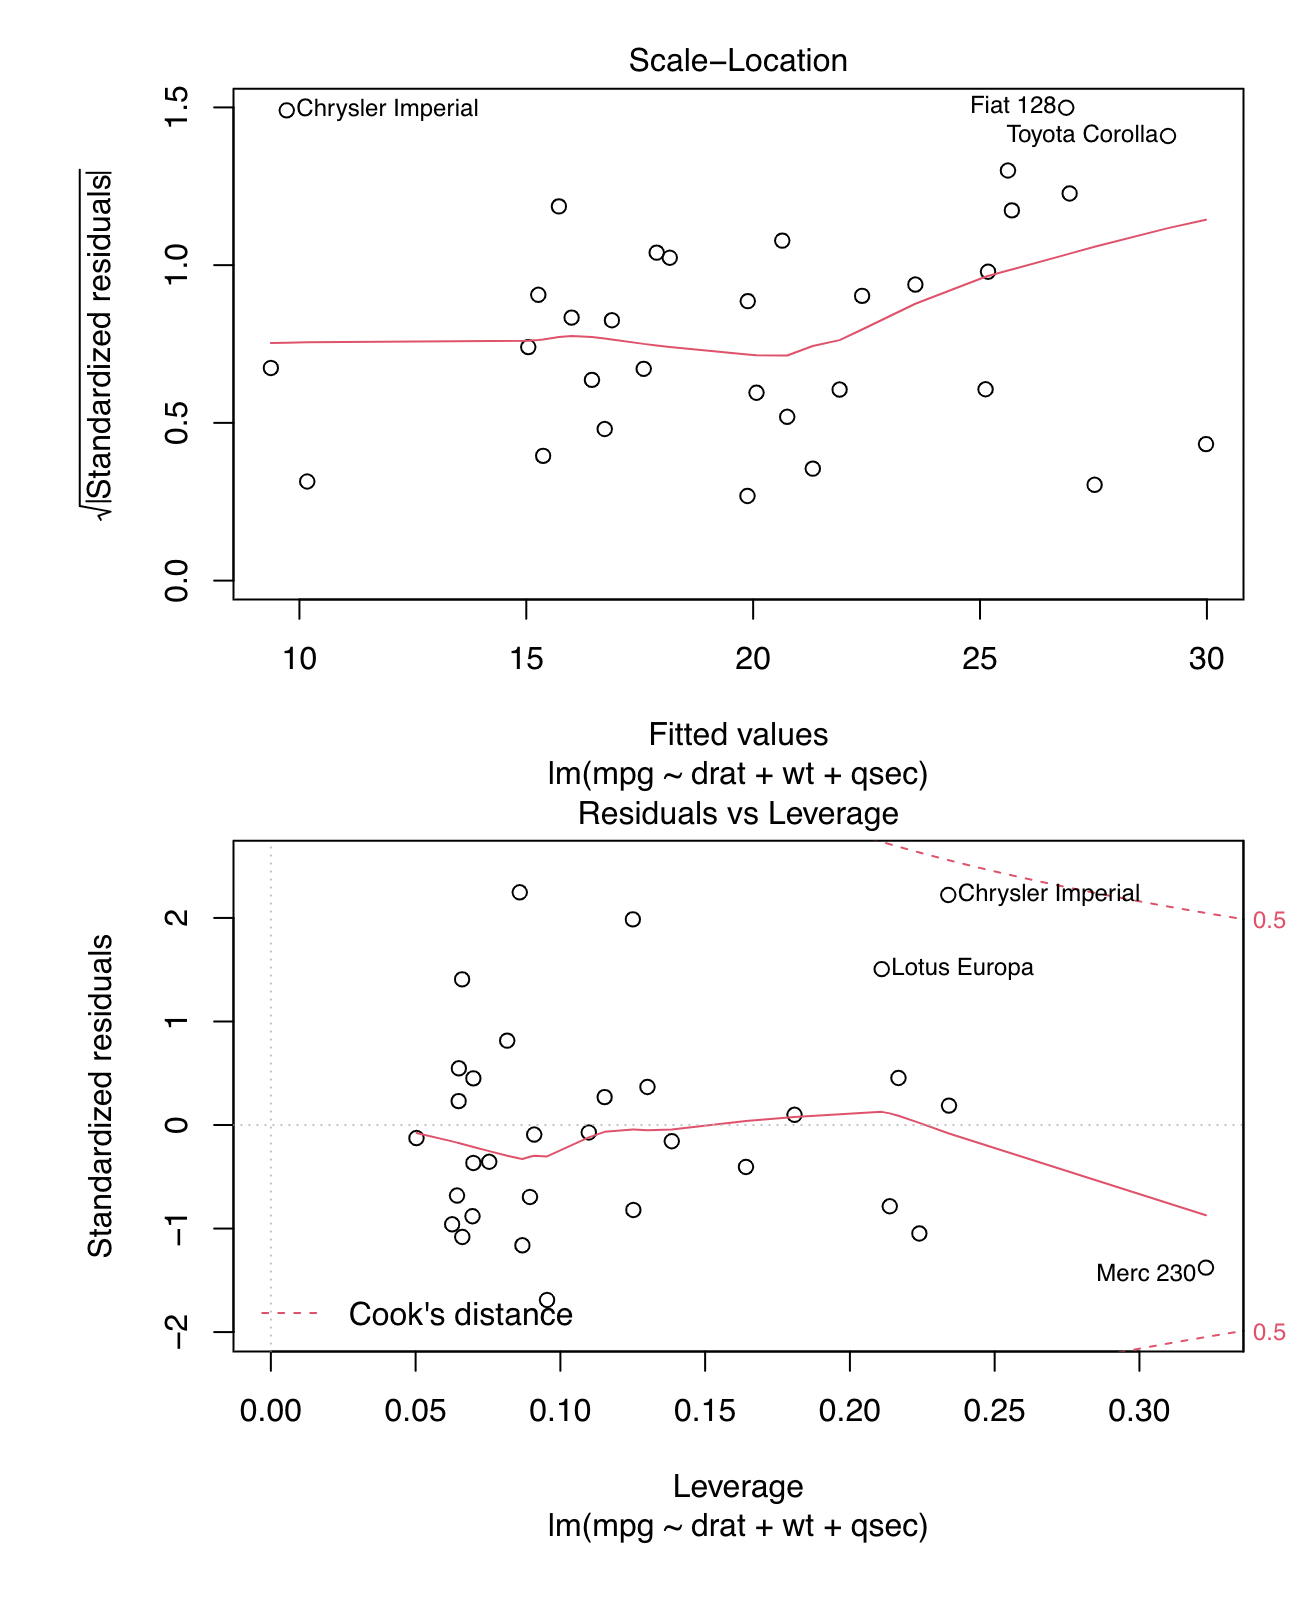
\includegraphics[width=0.9\textwidth]{Graph2} % second figure itself
    \end{minipage}
\end{figure}

\vspace{0.3cm}
\noindent The residuals vs fitted graph trend line is around 0. However,  the two end which trend downward(upward) at the start points(end points).  The start points does not seem to be a problem as indicated by the scale-location graph. However for the end point there seem to be a increasing variance which indicate we may not have a constant variances. \\

\noindent From the QQplots,  also reflect this as while the starting point not be perfectly normal they are close.  On the other hand,  the end points is not normally distributed .

\noindent The residuals vs leverage graph,  nothing really stand out, as point that may considered to be troublesome like Chrysler Imperial and Merc 230 are still with 0.5 crooks distance. 

\pagebreak

\noindent \textbf{Question 5:} Ridge Regression \\

\noindent \textbf{a.} Show the estimator: \\

\noindent Since $\sum_{i=1}^{n} e^2_i=(y-X\beta)^T(y-X\beta)$ and $\sum_{i=1}^{n}b^2_i=\beta^T\beta$.  The parameter  above is give by:

\begin{align*}
L(\beta)&=(y-X\beta)^T(y-X\beta)+\lambda(\beta^T\beta)\\
&=y^Ty-2y^TX\beta+\beta^T(X^TX)\beta+\lambda(\beta^T\beta)
\end{align*} 

\noindent To find the maximum likelihood estimator we find $\frac{\partial L}{\partial \beta}$ setting it to 0 then solve for $\beta$.

\begin{align*}
&\frac{\partial L}{\partial \beta} = 	-2(X^T y)+2 (X^T X) \beta+2 \lambda \beta=0 \\
&(X^TX+\lambda I)\beta=X^Ty \\
&\beta = (X^TX+\lambda I)^{-1}X^Ty
\end{align*}

\noindent Hence the estimator is give by $b=(X^TX+\lambda I)^{-1}X^Ty$. \\

\noindent \textbf{b.} Show that b is unbiased if $\lambda \neq 0$. \\

\begin{align*}
E(b)&=E(X^TX+\lambda I)^{-1}X^Ty) \\
&=(X^TX)^{-1}X^TE(y)+(\lambda I)^{-1}X^TE(y)\\
&=(X^TX)^{-1}X^TXb+(\lambda I)^{-1}X^TXb  & \text{Since E(y)=Xb}\\
&=b+(\lambda I)^{-1}X^TXb 
\end{align*} 

\noindent Since $(\lambda I)^{-1} X^TXb=0$ if and only if $\lambda = 0$ then $E(b) \neq b$ if $\lambda \neq 0$ hence it is biased when $\lambda \neq 0$.

\pagebreak
\noindent \textbf{c.} Optimal $\lambda$ value.

\begin{figure}[h]
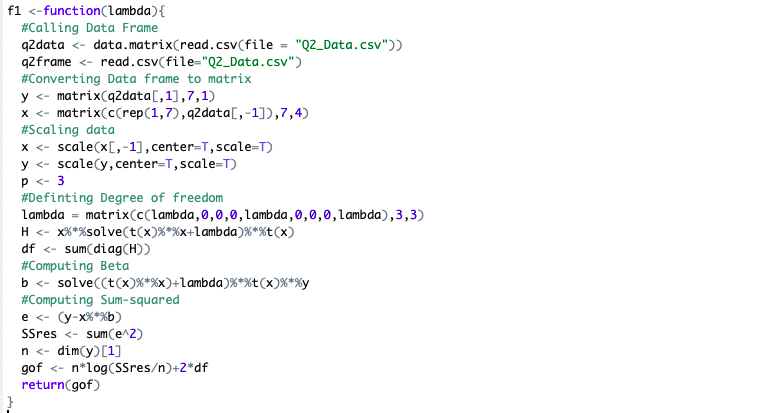
\includegraphics[scale=0.5]{q5}
\end{figure}

\begin{figure}[h]
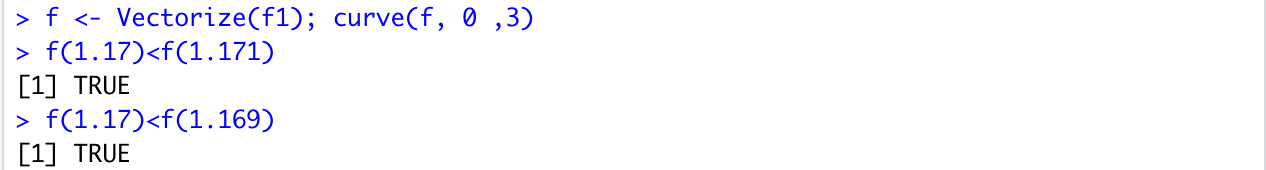
\includegraphics[scale=0.5]{graph4}
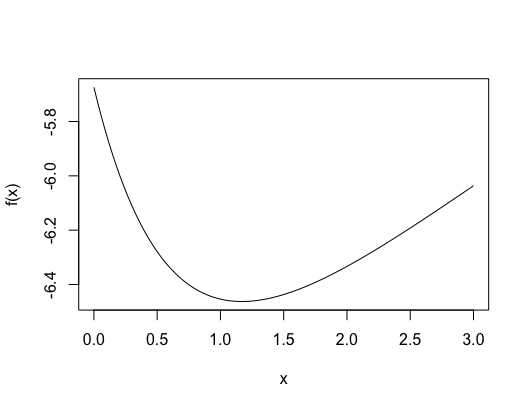
\includegraphics[scale=0.5]{graph3}
\end{figure}

Hence,  the optimal value for $\lambda$ is approximately 1.17.


\end{document}